% Home group worship songs
\documentclass[10pt,oneside,footinclude=true,headinclude=true]{scrbook} % KOMA-Script book
\usepackage[LHE,T1]{fontenc}
\usepackage[linedheaders,nochapters]{classicthesis} % ,manychapters
\usepackage[paperheight=11in,paperwidth=8.5in,margin=0.8in]{geometry}
\usepackage{graphicx}

\usepackage[english]{babel}

\usepackage{paracol}
\usepackage{transparent}
\usepackage{cancel}
\usepackage{tikz}
\usetikzlibrary{calc}

% Helper functions.
\makeatletter
\newcommand{\verbatimfont}[1]{\renewcommand{\verbatim@font}{#1}}
\makeatother

\newcommand\songtitle[1]{
	\hspace*{-3.7mm}\LARGE\textsc{#1}
}

\linespread{1.1}

\begin{document}

\verbatimfont{\rmfamily\Large}

%%---------------------------------------------------------------------------------------
%%	TITLE PAGE
%%---------------------------------------------------------------------------------------
%\begin{titlepage}
%\begin{center}
%\large \hfill \vfill
%
%\begingroup
%\color{RoyalPurple}\spacedallcaps{Dennis and Jus's} \\
%\bigskip
%\color{RoyalPurple}\spacedallcaps{\huge{Worship Songlist}} \\ %Title
%\bigskip
%\endgroup
%
%\bigskip\bigskip
%\bigskip\bigskip
%\bigskip\bigskip
%\bigskip
%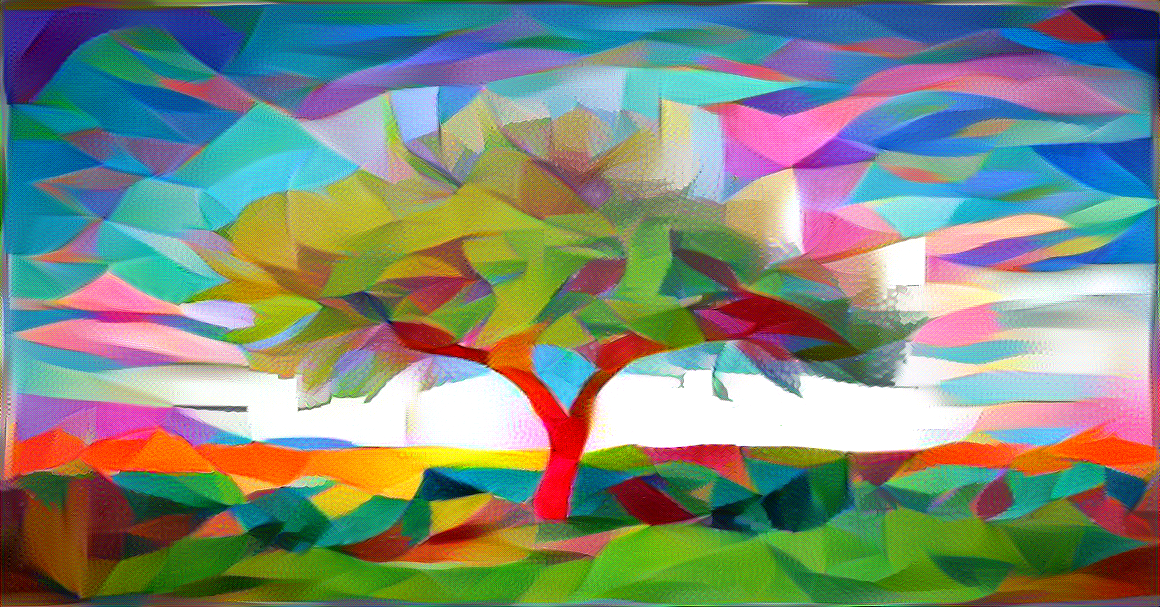
\includegraphics[width=10cm]{GSITree-triangle.png} \\
%\bigskip
%\bigskip\bigskip
%\bigskip\bigskip
%\bigskip\bigskip
%
%\textit{...The leaves of the tree were for the healing of the nations....} \\ \medskip % Subtitle
%
%January 2020\ -- version 1.0 % Time and version
%
%\vfill
%\end{center}
%\end{titlepage}
%    
%\pagenumbering{gobble}
%\pagenumbering{arabic}

%---------------------------------------------------------------------------------------
%	CHORDS
%---------------------------------------------------------------------------------------


%---------------------------------------------------------------------------------------
\verbatimfont{\ttfamily\large}

\newpage
\bigskip  
\songtitle{Chord Charts}
\begin{verbatim}

  You Are My All In All (Key of D)
  
  
D            A/C#               Bm7
  You are my strength when I am weak
              D/F#            G
  You are the treasure that I seek
             Asus4  D   A7
  You are my all in a-a-all
D             A/C#          Bm7
  Seeking you as a precious jewel
               D/F#        G
  Lord to give up I'd be a fool
             A7     D     A
  You are my all in all
  
  
  D   A/C#   Bm7     D/F#
  Je- sus,   Lamb of God
  Em7    D/F#    G   A7
  Worthy is your naa-me
  D   A/C#   Bm7     D/F#
  Je- sus,   Lamb of God
  G      Asus4   D      A
  Worthy is your name
  
  
D           A/C#            Bm7
  Taking my sin my cross my shame
          D/F#              G
  Rising again I bless your name
             Asus4  D   A7
  You are my all in a-a-all
D             A/C#             Bm7
  When I fall down you pick me up
            D/F#            G
  When I am dry you fill my cup
             A7     D
  You are my all in all
\end{verbatim}
\verbatimfont{\ttfamily\Large}
\newpage
\bigskip  
\begin{verbatim}

  Worthy, You Are Worthy (Key of A)
  
  
  A               Bm7              A/C#             D
  Worthy, you are worthy much more worthy than I know
  A          Bm7             A/C#           D
  I cannot imagine just how glorious you are
E              D             A/C#                D
  I cannot begin to tell how deep a love you bring
E                       D            A/C#                D   E/D
  Lord, my ears had heard of you but now my eyes have seen
  
  
         A             Bm7           A/C#     D
  You're worthy You're worthy You're worthy
         A            Bm7        A/C#       D
  You're worthy to be praised forever and a day
  
  
  A             Bm7          A/C#                D
  Glory, I give glory to the one who saved my soul
      A                   Bm7            A/C#                D
  You found me and you freed me from the shame that was my own
E              D             A/C#               D   E/D
  I cannot begin to tell how merciful you've been
E                       D            A/C#                D   E/D
  Lord, my ears had heard of you but now my eyes have seen
\end{verbatim}
\newpage
\bigskip  
\begin{verbatim}

  The Father's Song (Key of D)
  
  
D                 A/C#
  I have heard so many songs
D/C             G/B
  Listened to a thousand tongues
      Em7               Asus4                Bm7(b13)   Asus4
  But there is one that sounds above them all
D                        A/C#
  The Father's song, the Father's love
D/C                G/B
  You sung it over me, and for
   Em7          Asus4         D       Dsus2
  Eternity it's written on my heart
  
                  G          A/G
  Heaven's perfect melody
               D/F#          Bm13
  The Creator's    symphony
                  Em7        Asus4
  You are singing over me
               Bm7
  The Father's song
                  G          A/G
  Heaven's perfect mystery
                      D/F#             Bm13
  The King of Love has    sent for me
                     Em7     Asus4
  Now you're singing over me
               D
  The Father's song
\end{verbatim}

\end{document}
